\documentclass[aspectratio=169]{beamer}
\usepackage{beamerthemetot}
\usepackage{graphicx}
\usepackage{animate}
\usepackage{calligra}
\usepackage[absolute,overlay]{textpos}
\usepackage[T1]{fontenc}
\usefonttheme{professionalfonts}
\usepackage{tikz}
\usetikzlibrary{shapes,arrows}
\usepackage{xcolor}
\usepackage{mathtools}
\usepackage{cancel}
 

\newcommand{\mytitle}{\color{White}\huge{\textbf{New Machine Learning Strategies for Data Scarce Material Science Problems}}}
\newcommand{\mysubtitle}{\color{Pink}\Large{\textbf{Go/No-go Meeting}}}
\newcommand{\myauthor}{\color{White}\textcalligra{\LARGE Ozgur Taylan Turan}}
\newcommand{\authorlabel}{\small O.T. Turan}
\author{\authorlabel}
\usepackage[backend=bibtex,firstinits=true,maxnames=30,maxcitenames=20,url=false,style=authoryear]{biblatex}

\setlength\bibitemsep{0.3cm} % space between entries in the reference list
\renewcommand{\bibfont}{\normalfont\scriptsize}
\renewcommand{\cite}[1]{\footnote<.->[frame]{\fullcite{#1}}}
\setbeamertemplate{bibliography item}{}
\bibliography{../../../archive_bib/library.bib}


\begin{document}

\setbeamercovered{transparent}

{
\def\beamer@entrycode{\vspace*{-\headheight}}
\setbeamertemplate{frametitle}[default][center]
\setbeamertemplate{navigation symbols}{}
\usebackgroundtemplate{
\includegraphics[width=\paperwidth,height=\paperheight]{cover/coverart.pdf}}

\begin{frame}[plain] 

\begin{minipage}{\textwidth}
	\centering{\mytitle} \\
	%\vspace{1cm}
	%\centering{\mysubtitle} \\
	\vspace{1cm}
	\centering{\color{White}November 15, 2021} \\
	\vspace{1cm}
	\centering{\myauthor}\\
\end{minipage}
\end{frame}
}


\begin{frame}
  \centering
  \mysubtitle
\end{frame}

\begin{frame}{Outline}
  \centering
  \begin{itemize}
    \item Introduction 
    \item Literature
    \item Aim
    \item Research Questions
    \item Planning 
    \item Reflection 
  \end{itemize}
\end{frame}

%
% Meta Learning Definitions
%Learning to learn, also referred to as meta-learning, treats the training of a machine learning model as a learning problem in itself. In the context of this work if a machine learning model's performance on a task is improving with training experiences it is said to be learning. In the light of this definition a machine learning model is said to be learning to learn if the performance on each task improves with training experience obtained from each task and with the number of tasks \cite{thrun1998}. Meta-learning recently is being used to tackle few-shot learning problems, where there is little data available from the learning task that is of prime interest, whereas there is an abundance of data from other similar tasks. 

Learning to learn, also referred to as meta-learning, treats the training of a machine learning model as a learning problem in itself. In this setting, there exist multiple learning problems and the learning problems are treated altogether. Then, a machine learning model is said to be learning to learn if the performance on each task improves with training experience obtained from each task and with the number of tasks \cite{thrun1998}. Meta-learning recently is being used to tackle few-shot learning problems, where there is little data available from the learning task that is of prime interest, whereas there is an abundance of data from other similar tasks. 

% What Makes MAML Different
%Early works of the learning-to-learn paradigm relied upon the one supervisory and one sub-ordinate model that interacts with each other for meta-learning. On one hand, sub-ordinate models try to improve the performance with training examples and on the other hand, the supervisory model tries to increase the performance over the family of tasks. MAML (Model-Agnostic Meta-Learning) \cite{finn2017} is a model that circumvents the need for supervisory and subordinate models. This method tries to tackle meta-learning by training any (As the name suggests MAML applies to all learners that improve performance by SGD (Stochastic Gradient Descent).) machine learning models parameters in a way to maximize the performance on a new learning task with few experiences through one or more gradient steps. 

Early works of the learning-to-learn paradigm relied upon two consecutive models working simultaneously, where one model tries to improve performance on the specific task and the other tries to improve performance over the observed tasks together. Considering this nested structure  MAML (Model-Agnostic Meta-Learning) \cite{finn2017} provides an algorithm that circumvents the need for multiple models. This method tries to tackle meta-learning by training any (all learners that improve performance by SGD (Stochastic Gradient Descent)) machine learning models parameters in a way to maximize the performance on a new learning task with few experiences through one or more gradient steps. 

% Where to use MAML?
%MAML is used in few-shot learning problems in the supervised and reinforcement learning problems, where the losses differ from each other. Due to being model and problem independent MAML finds a wide application area in the context of few-shot meta-learning. Moreover, MAML also aims to improve a specific task performance quickly (with a few gradient steps). This is an additional aspect to our definition of meta-learning. 

Due to being model and problem independent MAML finds a wide application area in the context of few-shot meta-learning. It is used under few-shot learning problems for supervised and reinforcement learning problems, where the losses differ from each other.  Moreover, MAML also aims to improve a specific task performance quickly (with a few gradient steps). This is an additional aspect to the definition of meta-learning. 

% What is the problem?
%As mentioned above, MAML aims to improve the generalization of a model for a certain learning task from a given family of tasks, with little data and minimal training. Minimal training indicates quick adaptation capabilities. This feature can prove useful in certain settings, for instance, in robotics research, where the reaction/adaptation time of the agents to dynamic environments bestow an inherent time limitation. However, this limitation is not present for the supervised learning problems, where MAML or its variants are utilized as a baseline. (\eg \cite{flennerhag2019,nichol2018,rajasegaran2020,collins2020,guiroy2019} etc.) Most of the unsupervised problem benchmark is image detection problem, where $N$-way $K$-shot classification problem ($N$ different classes with $K$ labeled training data) is tried to be tackled. Given the nature of the problem, most of the time memory or time limitation does not constitute a major issue in the given problem setting.

MAML aims to improve the generalization of a model for a certain learning task from a given family of tasks, with little data and minimal training. Minimal training indicates quick adaptation capabilities. This feature can prove useful in certain settings, for instance, in robotics research, where the reaction/adaptation time of the agents to dynamic environments bestow an inherent time limitation. However, this limitation is not present for supervised learning problems, where MAML or its variants are utilized as a baseline. (\eg \cite{flennerhag2019,nichol2018,rajasegaran2020,collins2020,guiroy2019} etc.) Most of the unsupervised problem benchmark is image detection problem, where $N$-way $K$-shot classification problem ($N$ different classes with $K$ labeled training data) is tried to be tackled. Given the nature of the problem, most of the time memory or time limitation does not constitute a major issue in the given problem setting.

% What is our paper about?
The main aim of this paper is to investigate the MAML under the settings where quick adaptation is not needed, and where most of the applications and variants of this method are benchmarked. This will be achieved by looking at the expected performance of the MAML under two synthetic regression scenarios, and comparing its performance to conventional base learners (\eg Linear Regression, Ridge Regression, Kernel Ridge Regression, etc.). By doing this we aim to investigate the effect of the limited adaptation step, and whether or not there is a benefit to this limitation. % In the meantime, the effect of task variance, and noisy observations (unlike the setting presented in \cite{finn2017}) will also be investigated.



% Mechanics and computational power
The mechanics followed a deterministic approach for many years. This deterministic approaches helped humanity in various engineering and design problems. Over the last 5 decades engineering problems got increasingly complexer as the needs of the humanity changed in a similar fashion. These complex problems are tackled mostly with the combination of experimental and computer aided simulations until recently. In this combined endeavour, where experiments are hindered, computer aided simulations helped significantly eliminate the money and time limitations of the experimental approach. Especially due to increasing availability and accessibility of the computational power. Although, their wide spread use the deterministic high-fidelity numerical solutions, also known as computer aided simulations, requirement of time and money is also increasing as the complexity of the problems increase further. It is getting evidently clear that the Moore's Law is loosing its validity due to physical limitations of the silicone technology \cite{arenas2021}. Thus, if we want to continue solving complex problems in the coming future, the need for another approach that can further reduce the time and money requirements of the current experimental and computer aided numerical solutions.

% ML in mechanics
Machine learning (ML) applications from computer-vision, to speech-recognition are getting more and more essential part of our daily life. To this end, it is not a surprise that ML found use cases in mechanics as well. To the authors knowledge the first mechanics applications of the machine learning paradigm dates back to the second-boom (1990's till 2000's) of ML in the fields of civil and mechanical engineering (\eg \cite{reich1997,reich1995,bishop1993,adeli}). Similar to numerical method applications used in the field of mechanics, machine learning also benefited from the increasing computational power. However, to reach the popularity and wide-spread application areas can be attributed to the more open and development aimed attitude of the field. This increasing open-access to ML tools the applied use cases of the ML in the mechanics community started to flourish.

% Recent landscape
The effort put into decrease the time complexity of the direct numerical solutions, is sprouting. On one hand a general way to tackle the differential equations resulting in a mechanics problem is being tackled. For instance,  Physics-Informed Neural Networks (PINNs) \cite{raissi2019b} and it variants, where the fields of interests are represented as neural networks and the residual enforced by the differential equations, and initial and boundary conditions are minimized.  Moreover, the operators that are the key parts of differential equations are tried to be learn from the data in \cite{lu2021a}. On the other hand, more specific applications try to tackle more specific sub-problems with the help of various ML techniques. These examples mostly try to accelerate a certain part of a certain problem via data-driven approaches. Due to its nested structure the time complexity of the multi-scale direct numerical solutions are one of the most laborious endeavours in solid mechanics espcially when coupled with other physical-phenomenon. In \cite{bessa2017} one such application is shown where a multi-scale problem is tried to be tackled in micro-scale. Due to data hungry ML applications, another type of ML application, which is ML based reduced order models (\qg \cite{liu2016,ferreira2021}), are utilized. The utilization of these data hungry applications 

One of the major application areas involve the multi-scale 


% Problems with the landscape


% How can we solve these problems?


% The aim of the paper?


% Landscape of the current literature wrt our aim! 






\section{Literature}

\begin{frame}{FE$^2$ via Machine Learning}
  \begin{minipage}{0.5\textwidth}
  \only<1-2>
  {
    \centering
    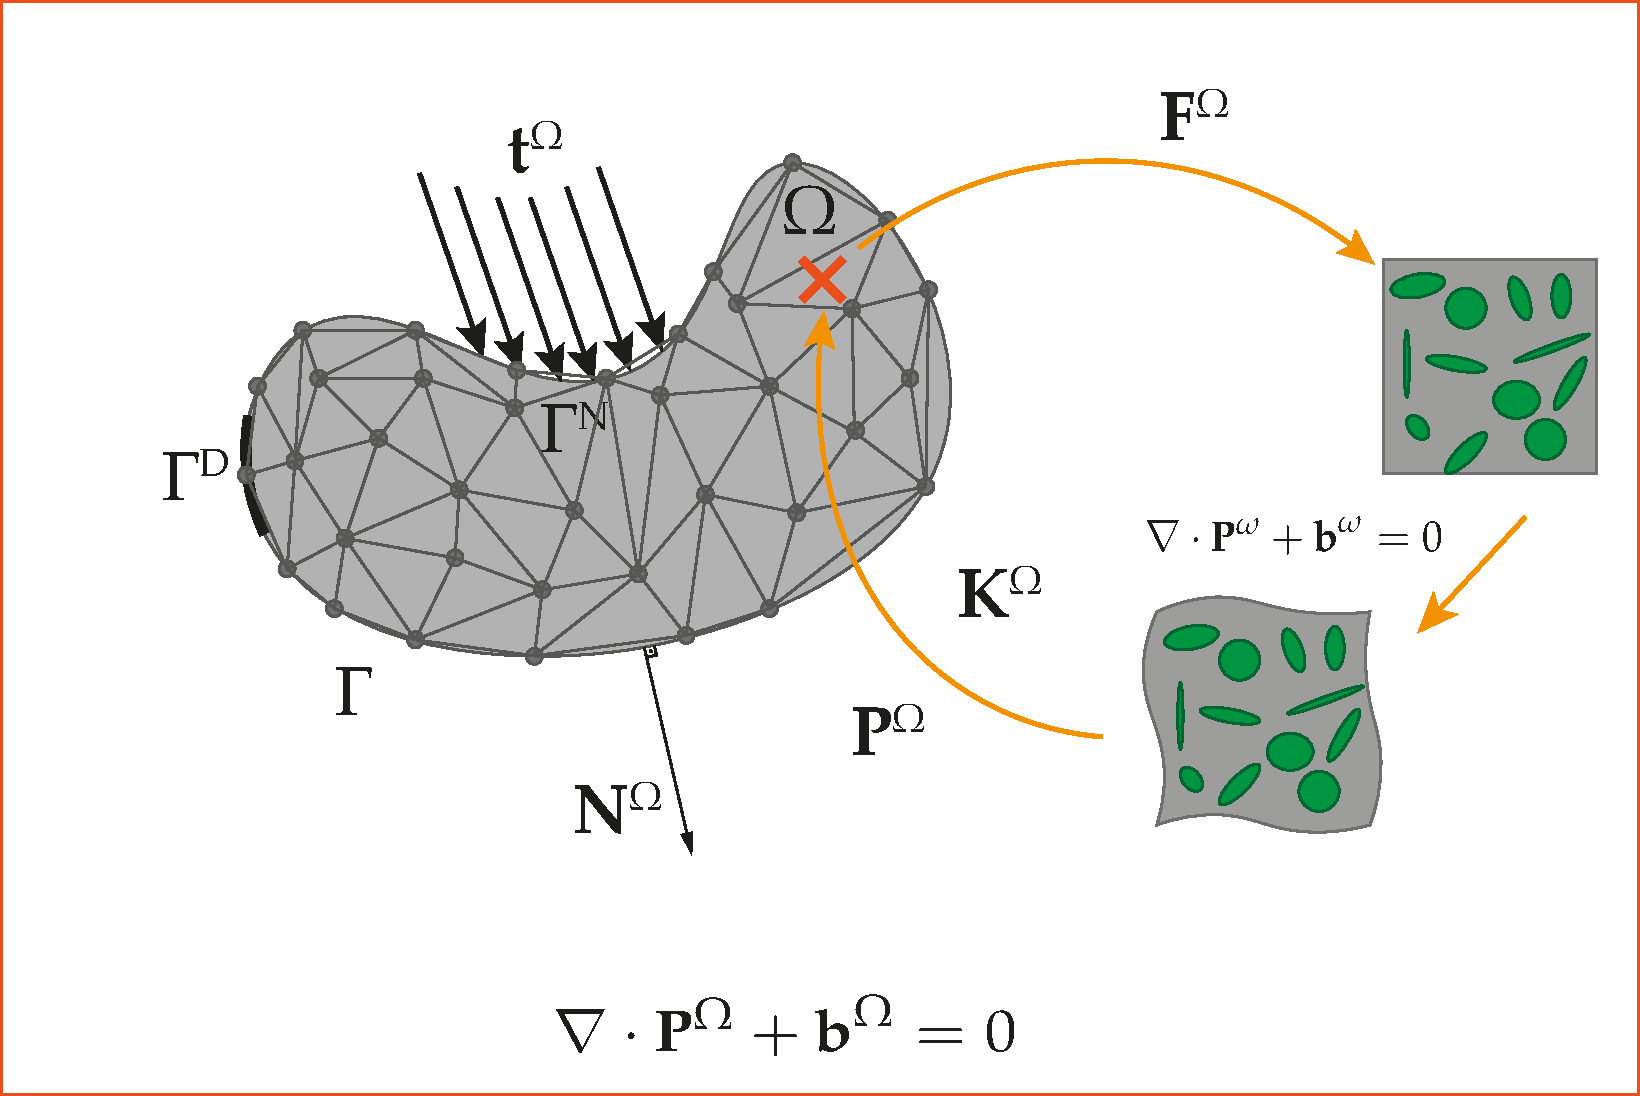
\includegraphics[width=0.9\textwidth]{Figures/intro/FE2-CONV}
  }
  \only<3>
  {
    \begin{block}{\color{White} Problems in Current State}
      \begin{itemize}
        \item Risky Extrapolation
        \item Data Scarcity
        \item Single Parameter Configuration
        \item General Applicability
      \end{itemize}
    \end{block}
  
  }
  \end{minipage}%
  \begin{minipage}{0.5\textwidth}
  \only<1-3>
  {
    \centering
    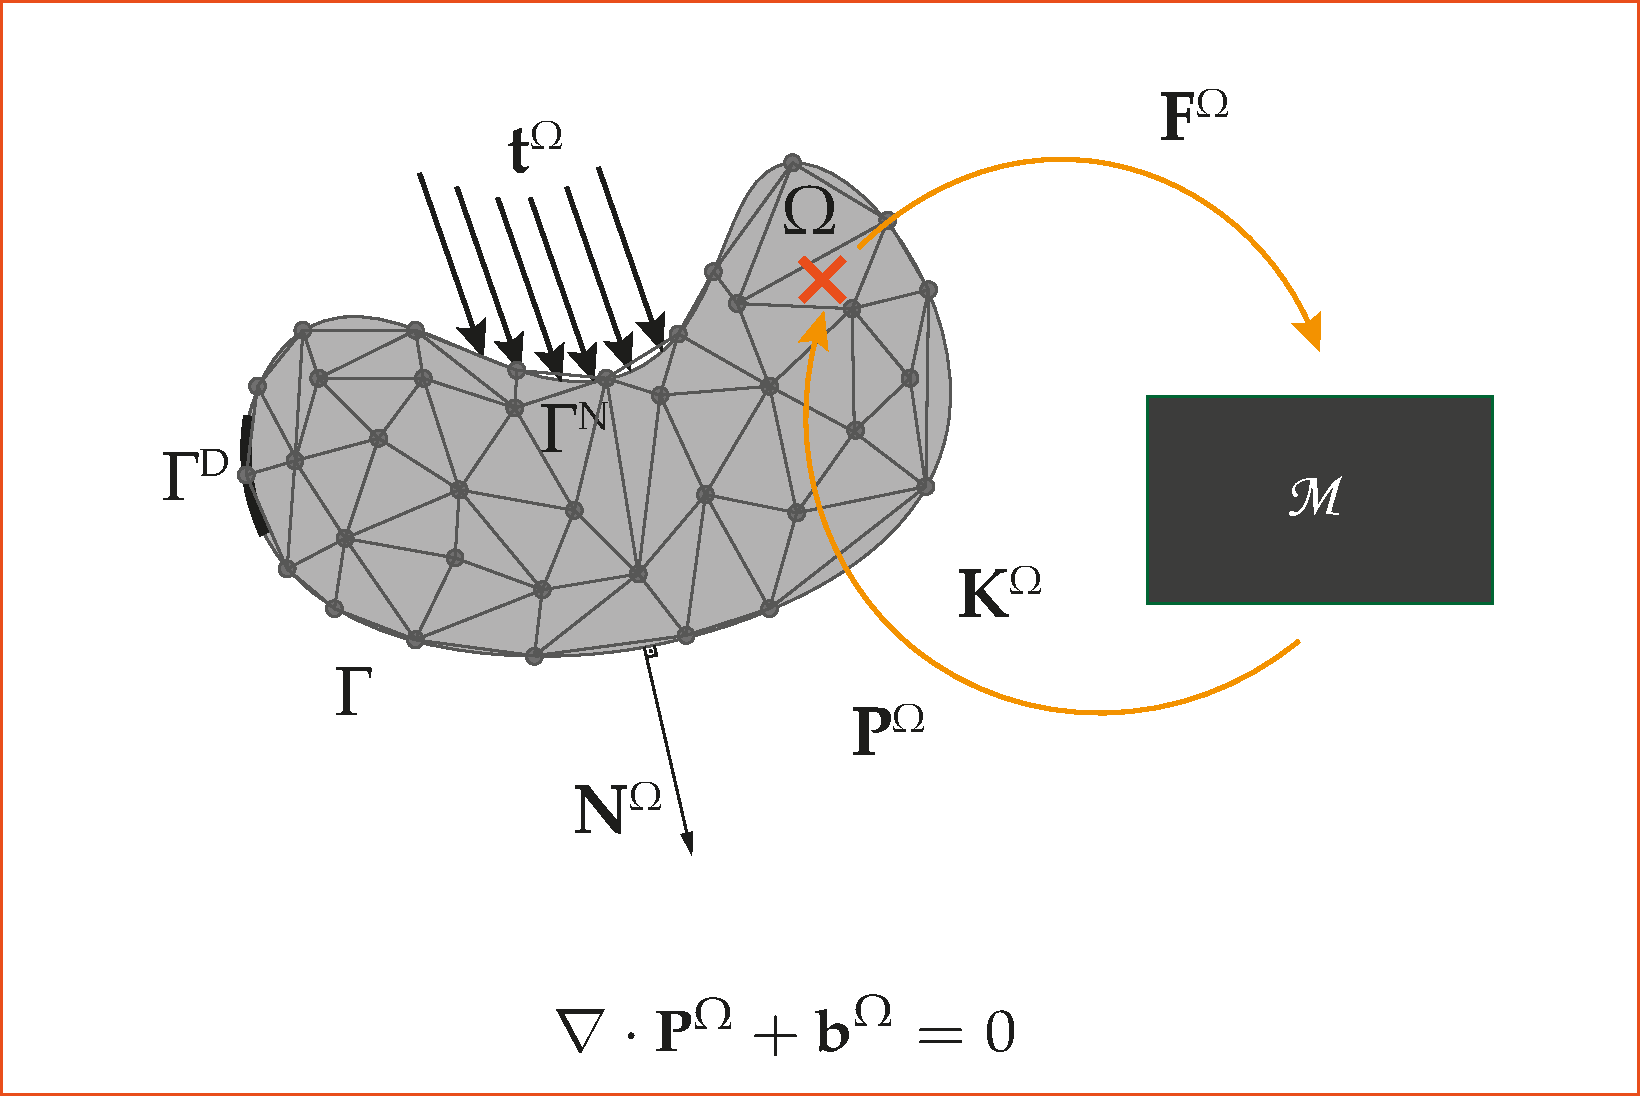
\includegraphics[width=0.9\textwidth]{Figures/literature/FE2-ML}
  }
  \end{minipage}
\only<2>
{
  \begin{itemize}
  \centering
    \item \color{Pink} Computationally a Material: $\mathbf{F} \to \mathbf{P}$
  \end{itemize}
}
\end{frame}

\begin{frame}{Hypothesis}
  \begin{itemize} 
    \item Most of the problems encountered can be tackled with more general approaches.
    \item The core problem is finding the mapping between a deformation measure and a force measure. ($\mathbf{P}=\mathcal{C}(\mathbf{F})$).
    \item Similarity between the problems can be exploited, without considering the different parameters that effect the model.
  \end{itemize}
\end{frame}







To formalize our supervised learning problem setting let us start by introducing generic input and output spaces as $\ispace$ and $\ospace$. A learning algorithm $\algo$ takes i.i.d samples $\samp:=(\inp,\out)_{i=1}^{N}$ (also represented by$\algo(\samp)$), from an unknown distribution $\prob_{\samp}$ over $\ispace \times \ospace$ and produces a hypothesis $\hyp$ from hypothesis class $\hypspace$ defined by the learner $\algo$. Then, the prediction of a learner can be represented as $\pred=h(\inp)\in\ospace$. Moreover, the performance of the learner is measured by a loss function $\loss(\out,\pred)$. Thus, the expected loss or risk $\risk$ of a hypothesis generated by a learning algorithm over the true distribution $\prob_{\samp}$ is given as:

\begin{equation}
 \risk(\hyp) = \int\loss(\out,\pred)d\prob_{\samp}.
\end{equation}

%Noting that the loss used to calculate the risk does not need to be the same loss utilized in the training of the learner. 

A reliable learning curve of a learner is obtained by averaging over many $\samp$ for varying $\nsamp$. Then, the average risk of a learner is given as:
\begin{equation}
 \avgrisk(\algo, \nsamp) = \underset{{\samp}}\expect\risk(\algo(\samp))).
\end{equation}

An individual learning curve $\lc:\R\to\R$ depends on $\algo$ and $\prob_{\samp}$. This allows us to represent this as a supervised learning problem. Let us assume that predicting a learning curve is the task $\task_i$ that we are interested in and we are given training size and corresponding risk values from this curve $\samplr:=(\nsamp_i,\risk_i)_{i=1}^{\nsamplr}$ and learning curves $(\lc_i)_{i=1}^\numlc$. Note that the curves are not analytical but in a discretized point-wise available. As mentioned before the cost of obtaining a learning curve increases as the $\nsamp$ increases. Thus, we assume that $\nsampi\subset[0,\nlim]$ where $\nlim\in\Zpos$, but limited to be small, so that the cost of obtaining $\risk(\algo(\sampi))$ is not large. In other words, we are trying to model $\lc$ by training a learner $\model:\R\to\R$ with samples $\samplr$ and $(\lc_i)_{i=1}^\numlc$.

It should be noted that in most cases the true distribution of the data is unknown, thus the empirical version of the risk is obtained by creating one hold-out set and several cross-validation splits. Moreover, additional splits might be necessary if the hyper-parameters of the learner are to be tuned as well. 



\section{Research Questions}
\begin{frame}{Research Questions}
  %\color{Pink} Prediction of a mapping $\mathcal{T}_{\mathcal{A}^\prime}$ given a batch of mappings $\{\mathcal{T}_{\mathcal{A}_i}\}_{i=1}^{M}$ where $\mathcal{A}^\prime \in \boldsymbol{\mathcal{A}}$
  \begin{itemize}
    \item To what extent this prediction is possible?
    \item Can we find a latent space where the tasks with different parameters live and exploit the similarities between these tasks?
    \item What information can we extract from the model trained with the batch of tasks at hand?
    \item Can we find an effective sampling strategy in the task space and in the feature space of the given task?
  \end{itemize}
\end{frame}

\begin{frame}{Related Paradigms in ML Literature}
  \begin{itemize}
    \centering
    \item \color{Pink} Meta Learning (Learning-to-learn) \color{Black}
    \item Transfer Learning and Domain Adaptation
    \item Multi-task Learning
  \end{itemize}
\end{frame}


\section{Planning}

\begin{frame}{Project Planning}
  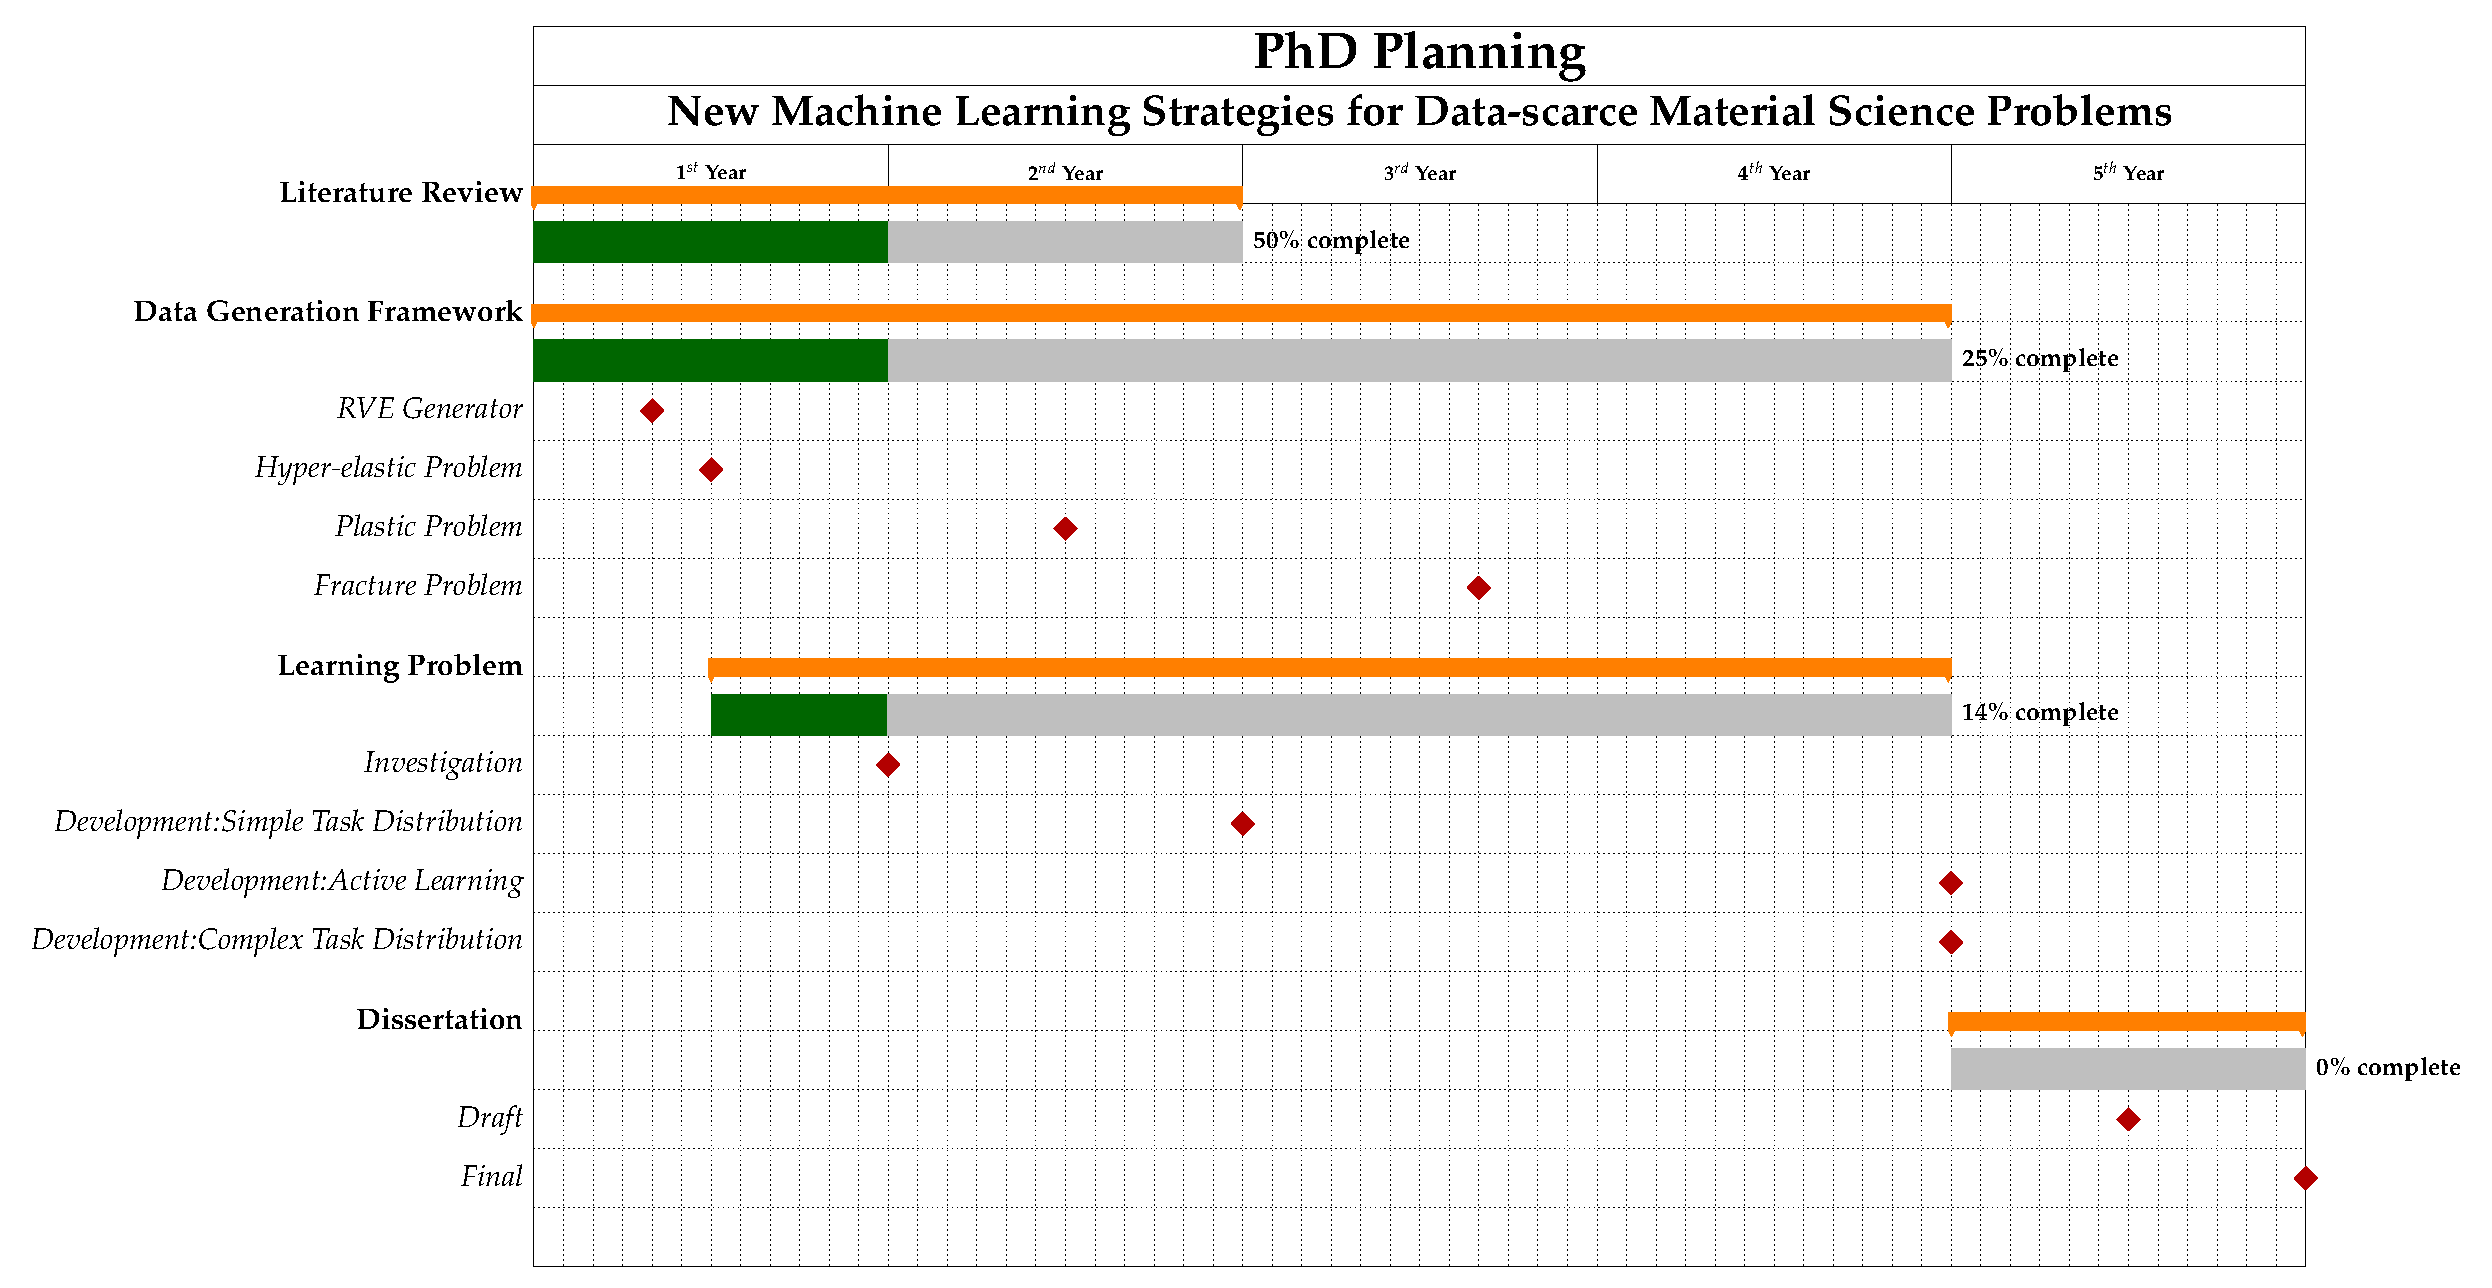
\includegraphics[width=0.85\textwidth]{Figures/planning/project_plan}
\end{frame}

\begin{frame}{Collaborations}
  \begin{itemize}
    \item Continuation of my MSc. Thesis Multi-fidelity Gaussian Process Regression 
    \item Miguel Bessa and I in collaboration with Iuri Rocha and Frans van der Meer from Civil Engineering and Geosciences  
    \item Data Generation
  \end{itemize}
\end{frame}

\begin{frame}{Doctoral Education Planning}
\centering
  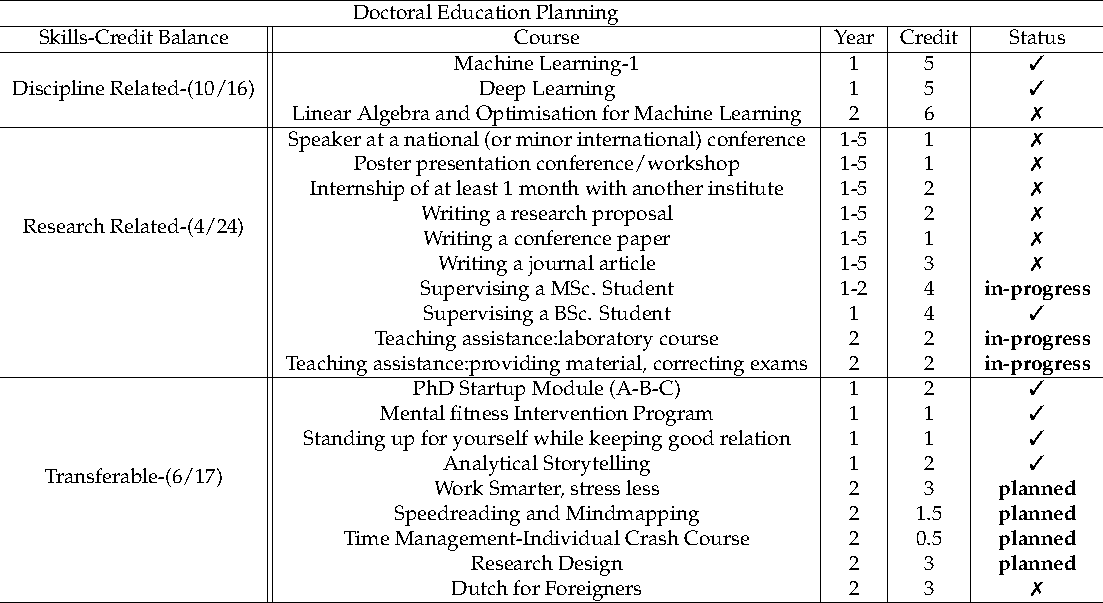
\includegraphics[width=0.8\textwidth]{Figures/planning/doctoral_education_plan}
\end{frame}



\section{Reflection}
\begin{frame}{Past Year with COVID19}
  \begin{minipage}{0.45\textwidth}
    \begin{block}{\color{White} Academic}
      \begin{itemize}
        \item PRB 
        \item Collaboration
      \end{itemize}
    \end{block}
  \end{minipage}%
  \hspace{5mm}
  \begin{minipage}{0.45\textwidth}
    \only<2>
    {
    \begin{block}{\color{White} Non-Academic}
      \begin{itemize}
        \item Work-Life Balance
        \item Well-being
      \end{itemize}
    \end{block}
  }
  \end{minipage}
\end{frame}

\begin{frame}
  \centering
  \color{Pink} Thanks for your attention!
\end{frame}
\section{Extras}
\begin{frame}{Reformulate the Problem-\only<1>{A}\only<2>{B}}
  \begin{minipage}{0.5\textwidth}
\only<1>
{
    \begin{block}{\color{White} $\mathbf{P}=\mathcal{C}(\mathbf{F})$}
      \begin{itemize}
        \item Normally, $\mathbf{P}=f(\mathbf{F}, \boldsymbol\gamma)$
        \item $\boldsymbol{\gamma}:=\{\gamma_i\}_{i=1}^{M}$ with $M\in\mathbb{Z}^+$
        \item $\mathbf{P}=\mathcal{M}(\mathbf{F}, \boldsymbol{\gamma})$
        \item Application specific models! 
      \end{itemize}
    \end{block} 
}
\only<2>
{
    \begin{block}{\color{White} $\mathbf{P}=\mathcal{C}(\mathbf{F})$}
      \begin{itemize}
        \item Let's stick to $\mathbf{P}=\mathcal{C}(\mathbf{F})$
        \item Then, $\mathbf{P}=\mathcal{M}(\mathbf{F})$
      \end{itemize}
    \end{block} 
    \begin{block}{\color{White} How to account for $\boldsymbol{\gamma}$?}
      \begin{itemize}
        \item Let's stick to $\{\mathbf{P}_i=\mathcal{C}_i(\mathbf{F})\}_{i=1}^{M}$ with $M\in\mathbb{Z}^+$
        \item $\mathbf{P}=\mathcal{M}(\mathbf{F})$
        \item Model input-output remains the same!
      \end{itemize}
    \end{block} 
}
  \end{minipage}%
  \begin{minipage}{0.5\textwidth}
    \centering
    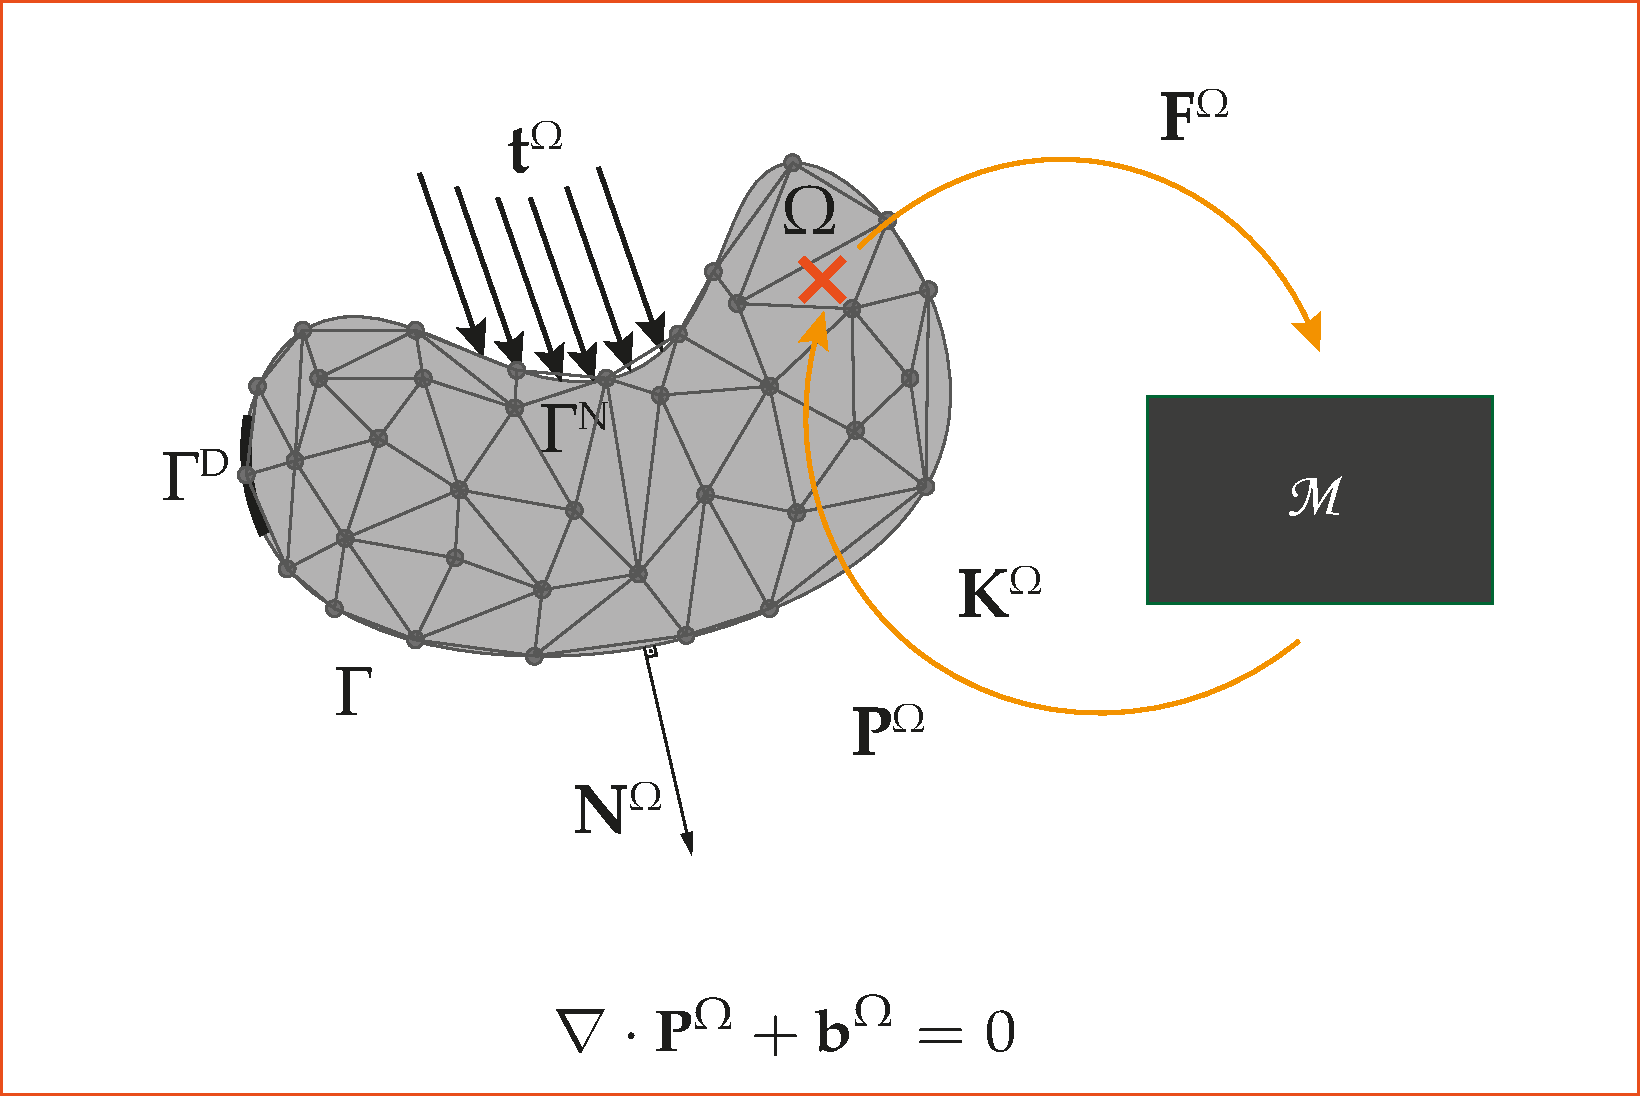
\includegraphics[width=0.9\textwidth]{Figures/literature/FE2-ML.pdf} 
  \end{minipage}
\end{frame}

\begin{frame}{Reformulate the Problem-\only<1>{C}\only<2>{D}}
  \begin{minipage}{0.5\textwidth}
\only<1>
{
    \begin{block}{\color{White} How do we end up with a parametrized relationships?}
      \begin{itemize}
        \item Series of assumptions, $\mathcal{A}:\{a_n \subset a_{n-1} \subset ... \subset a_1\}$ 
     \end{itemize}
    \end{block} 
    \begin{block}{\color{White} Individual Learning Problem}
      \begin{itemize}
        \item If the aim is to learn $\mathbf{F} \to \mathbf{P}$ 
        \item Learning problem: $\mathcal{T}_\mathcal{A}:\mathbf{F} \to \mathbf{P}$
      \end{itemize}
    \end{block}
}
\only<2>
{
    \begin{block}{\color{White} Overall Learning Problem}
      \begin{itemize}
        \item Given $\{\mathbf{P}_i=\mathcal{C}_i(\mathbf{F})\}_{i=1}^{M}$ with $M\in\mathbb{Z}^+$
        \item Learning problem: $\{\mathcal{T}_{\mathcal{A}_i}:\mathbf{F} \to \mathbf{P}_i\}_{i=1}^{M}$
      \end{itemize}
    \end{block} 
}
  \end{minipage}%
  \begin{minipage}{0.5\textwidth}
    \centering
    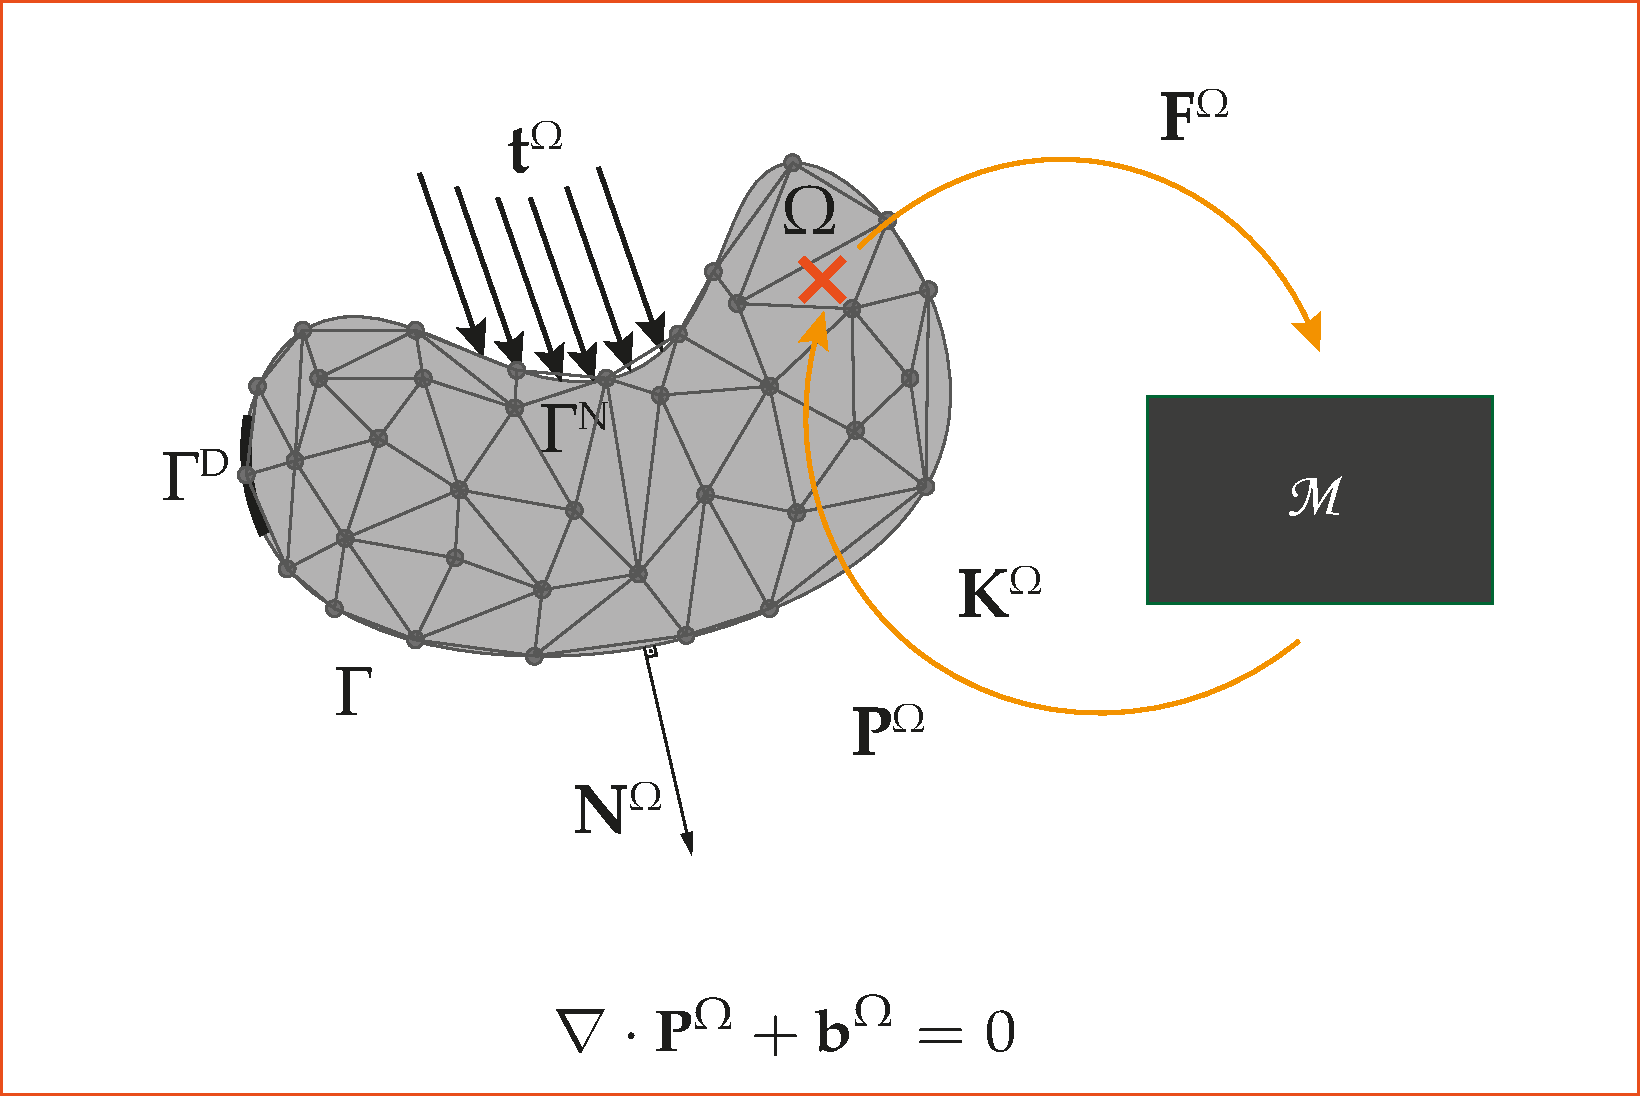
\includegraphics[width=0.9\textwidth]{Figures/literature/FE2-ML.pdf} 
  \end{minipage}
\end{frame}

\begin{frame}{Single-Task Learning vs Bias Learning-\only<1>{A}\only<2>{B}}
  \only<1>
  {
    \begin{block}{\color{White} Single-Task Learning}
      \begin{itemize}
        \item Input Space $\mathbf{F}$ OutputSpace $\mathbf{P}$
        \item Probability Distribution $p$ on $\mathbf{F}\times\mathbf{P}$
        \item Loss Function $l:\mathbf{P}\times\mathbf{P}\to \mathbb{R}$
        \item Hypothesis Space $\mathcal{H}$, a set of functions $h:\mathbf{F}\to\mathbf{P}$
        \item Minimize the expected loss to get $h\in\mathcal{H}$
      \end{itemize}
    \end{block}
  }
  \only<2>
  {
    \begin{block}{\color{White} Bias  Learning}
      \begin{itemize}
         \item Input Space $\mathbf{F}$ OutputSpace $\mathbf{P}$
        \item Probability Distribution $p$ on $\mathbf{F}\times\mathbf{P}$
        \item Loss Function $l:\mathbf{P}\times\mathbf{P}\to \mathbb{R}$
        \item An environment $(\mathcal{Q},\mathcal{P})$ where $\mathcal{P}$ is all possible distribution of $p$ and $\mathcal{Q}$ is the distribution of $\mathcal{P}$
        \item Hypothesis Space Family $\mathbb{H}:=\{\mathcal{H}\}$, where each $\mathcal{H}$ is a set of functions $h:\mathbf{F}\to\mathbf{P}$
        \item Minimize the expected future risk or transfer risk to find the appropriate Hypothesis Space $\mathcal{H}$ 
      \end{itemize}
    \end{block}
  }
\end{frame}

\begin{frame}{MAML vs Multi-task}
	\begin{itemize}
		\item Problem: $y=a*\text{sin}(x+p)$ for $x\in[0,5]$ and $a\in[0.1,5]$ \& $a\in[0,\pi]$ for $\text{K}=5$ and $\mathcal{B}(\mathcal{T})$ size $100$
	\end{itemize}
	\begin{minipage}{0.5\textwidth}
		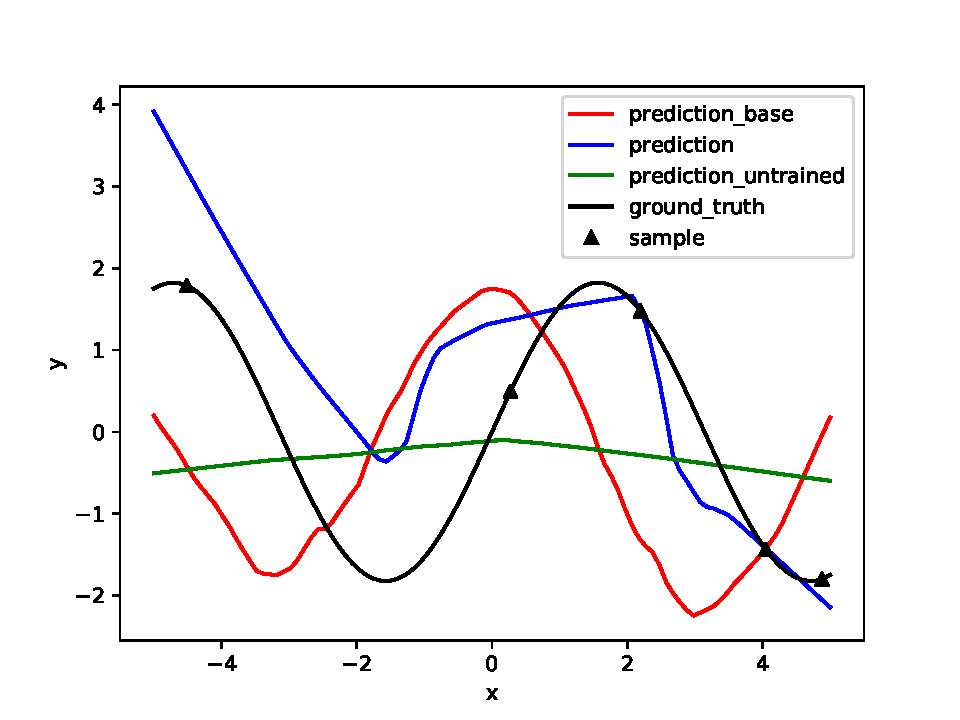
\includegraphics[width=0.9\textwidth]{Figures/Study1/sine-hard-finn-maml-pred.pdf}
		\centering
			MAML
	\end{minipage}%
	\begin{minipage}{0.5\textwidth}
		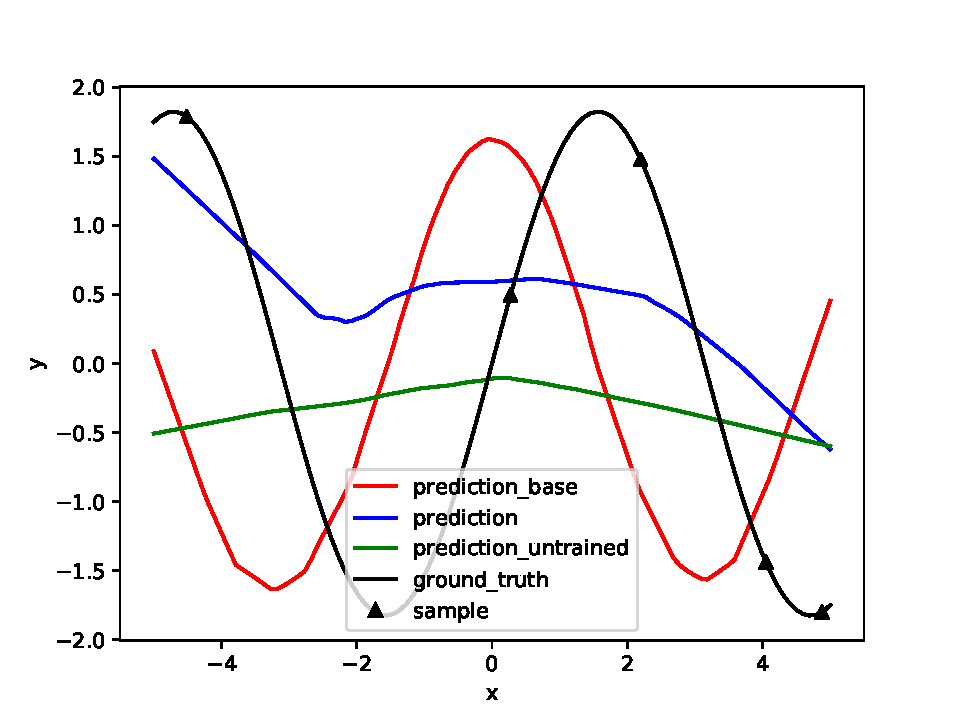
\includegraphics[width=0.9\textwidth]{Figures/Study1/sine-hard-finn-multitask-pred.pdf}
		\centering
			Multi-task
	\end{minipage}
\end{frame}

\begin{frame}{Small Investigation of MAML \cite{Finn2017}}
  \begin{minipage}{0.5\textwidth}
    \begin{itemize}
      \item $ a \in \mathbb{R}^d \to p_a \sim \mathcal{N}(m\mathbf{1},c\mathbf{I})$
      \item $ x \in \mathbb{R}^d \to p_x \sim \mathcal{U}(\mathbf{0},b\mathbf{1})$
      \item $ \varepsilon \sim \mathcal{N}(0,\sigma^2)$
      \item $ y = a^\text{T}x + \varepsilon \quad \in \mathbb{R}$
      \item $ Z:= ((x_i,y_i))_{i=1}^N$
      \item $ \hat{a}_N \to $ an estimator trained with N training points
    \end{itemize}
  \end{minipage}%
  \begin{minipage}{0.5\textwidth}
    Expected Error over the whole task space,
      $ \int \int \int (\hat{a}_N(Z)^{\text{T}}x-y)^2p(x,y)dxdyp_ZdZp_ada$
  \end{minipage}
  \color{Pink} Investigating the performance of a future emprical risk minimizing algorithm for transfer risk.
\end{frame}

\begin{frame}{F3DASM}
\centering
\begin{minipage}{0.55\textwidth}
		\begin{itemize}
		\item Design of Experiements
		\item Simulation or Machine Learning Module
	\end{itemize}	
\end{minipage}

\begin{minipage}{0.4\textwidth}
	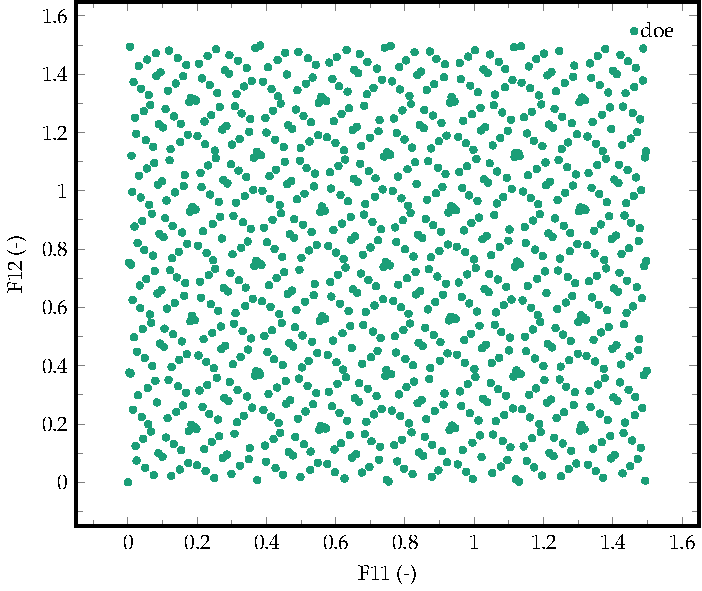
\includegraphics[width=\textwidth]{Figures/F3DASM/doe}
\end{minipage}%
\hspace{1mm}$\xRightarrow{\text{FEM}(\mathbf{F})}$
\begin{minipage}{0.4\textwidth}
	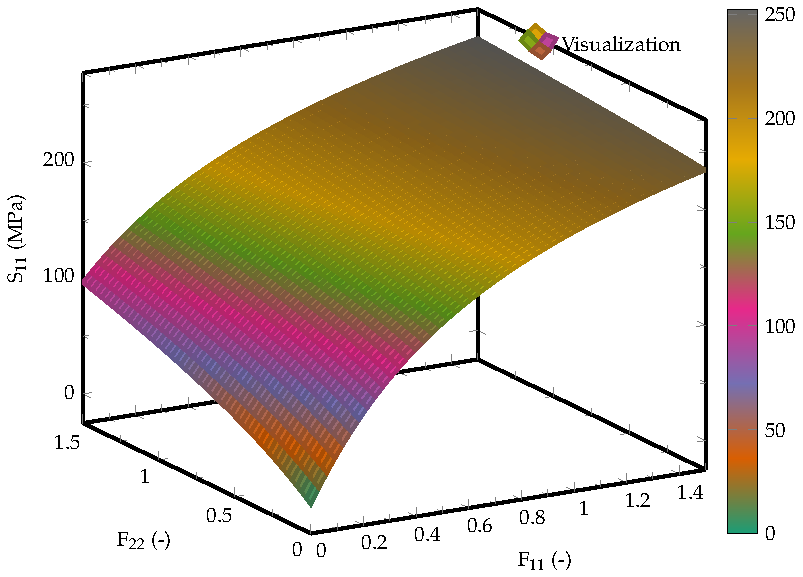
\includegraphics[width=\textwidth]{Figures/F3DASM/manifold}
\end{minipage}%
\end{frame}

\begin{frame}{Summer Schools \& Conferences}
\only<1>
{
  \begin{block}{\color{White} Summer Schools}
  \begin{itemize}
    \item Machine Learning Summer Schools (MLSS)
    \item Gaussian Process Summer School 
    \item Nordic Probabilistic AI Summer School
    \item Oxford Machine Learning Summer School
  \end{itemize}
  \end{block}
}
\only<2>
{
  \begin{block}{\color{White} Conferences on ML}
  \begin{itemize}
    \item Conference on Computer Vision and Pattern Recognition (CVPR)
    \item International Conference on Learning Representations (ICLR)
    \item International Conference on Machine Learning (ICML)
    \item International Conference on Machine Learning and Pattern Recognition (ICMLPR)
  \end{itemize}
  \end{block}
}

\only<3>
{
  \begin{block}{\color{White} Conferences on Mechanics}
  \begin{itemize}
    \item FEniCS Conference
    \item International Conference on Mathematics and Computational Mechanics (ICMCM)
    \item International Conference on Computational Geomechanics and Material Response (ICCGMR)
    \item FEniCS Conference
    \item International Conference on Computational Continuum Mechanics and Dynamics (ICCCMD)
\item International Conference on Computational Continuum and Continuum Mechanics (ICCCM)
  \end{itemize}
  \end{block}
}
\end{frame}





\end{document}
